\documentclass[a4paper, 11pt,table]{article}

\usepackage[utf8]{inputenc}
\usepackage[T1]{fontenc}
\usepackage[toc,page]{appendix}
\usepackage{varioref}
\usepackage{hyperref}
\usepackage[nameinlink]{cleveref}
\usepackage{nameref}
\usepackage{parskip}
\usepackage{multicol}%multi column bib
\usepackage[sectionbib, tocbib, numberedbib, bibnewpage]{apacite}%Citations
\usepackage{tikz}
\usepackage{pdflscape}
\usepackage{tabu}
\usepackage{pgfplots}
\usepackage[margin=0.6in]{geometry}
\usepackage[compact]{titlesec}

\usepackage{comment}
%\excludecomment{figure}
%\let\endfigure\relax

\pagenumbering{gobble}

\author{Steven Lowes}
\title{Software Methodologies AI Search}
\date{\today{}}

\newcommand{\smartref}[1]{%
	\hyperref[#1]{\cref{#1}, ``\nameref{#1}", \vpageref{#1}}%
}

\begin{document}
	
	\section{Algorithm A: Simulated Annealing}
	
	\subsection{Description}
	\begin{tabu}{p{10cm} X[c]}
		Simulated Annealing is similar to a hill climbing algorithm, except it will occasionally move to a worse state. The chance of doing so decreases as the algorithm nears completion. The algorithm randomly selects a neighbouring state, and moves to that state with a chance of:
		
		\begin{equation}
		e^{\frac{currentValue - newValue}{T}}
		\end{equation}
		
		T (temperature) is set with a parameter at the start of the algorithm, and decreases exponentially until it reaches the end temperature, also set by a parameter. The rate of decrease is set by another parameter, called the cooling rate.
		&
		\rowcolors{0}{gray!25}{white}
		\begin{tabu}{|c c|}\hline
			\textbf{Nodes} & \textbf{Tour Length} \\
			12 & 56.0 \\
			17 & 1,514 \\
			21 & 2,668 \\
			26 & 1,479 \\
			42 & 1,217 \\
			48 & 13,999 \\
			58 & 26,740 \\
			175 & 21,519 \\
			180 & 2,540 \\
			535 & 49,007 \\\hline
		\end{tabu}
	\end{tabu}
	
	\subsection{Start/End Temp}
	When the Start Temperature is too high, the simulation will frequently jump to worse states in the beginning. This means that the algorithm does not even begin to converge until it is a significant way through, wasting lots of computation. If the starting temperature is too low, the algorithm will get stuck in local minima.
	
	When the End Temperature is very low, the algorithm will spend a long time in a local minima, looking for a better result without ever jumping to a worse result, wasting computation time. If the End Temperature is too high, it will never properly descend into the local minima.
	
	In each test, the cooling rate was set so that the number of steps remained at 1,000,000. This was deliberately low, so that the effects of changing the start and end temperatures were exaggerated. It was found that a start temperature of 80 and an end temperature of 0.5 were optimal.
	
	
	\begin{tabu}{X[c] X[c]}		
		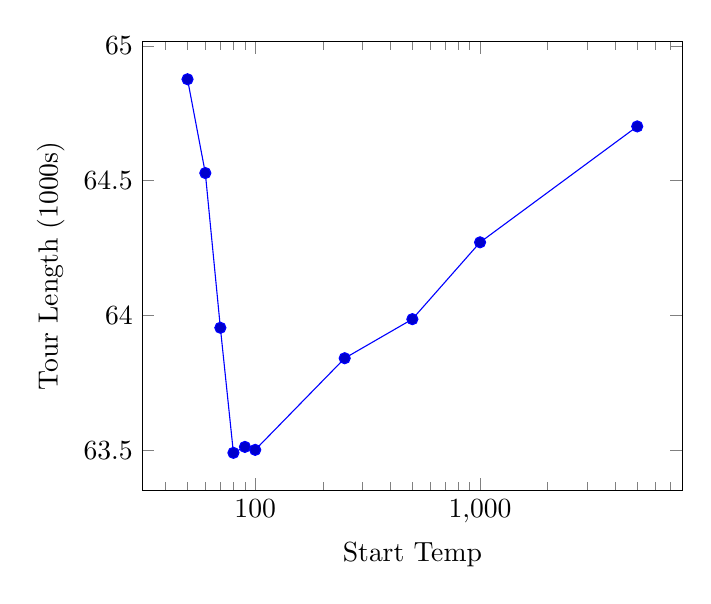
\begin{tikzpicture}
		\begin{axis}[
		%title = Effects of changing start temp,
		xlabel = {Start Temp},
		ylabel = {Tour Length (1000s)},
		xmode=log,
		log ticks with fixed point,
		]
		\addplot coordinates {
			(50,64.876)
			(60,64.528)
			(70,63.954)
			(80,63.490)
			(90,63.512)
			(100,63.501)
			(250,63.841)
			(500,63.986)
			(1000,64.271)
			(5000,64.701)
		};
		\end{axis}
		\end{tikzpicture}&
		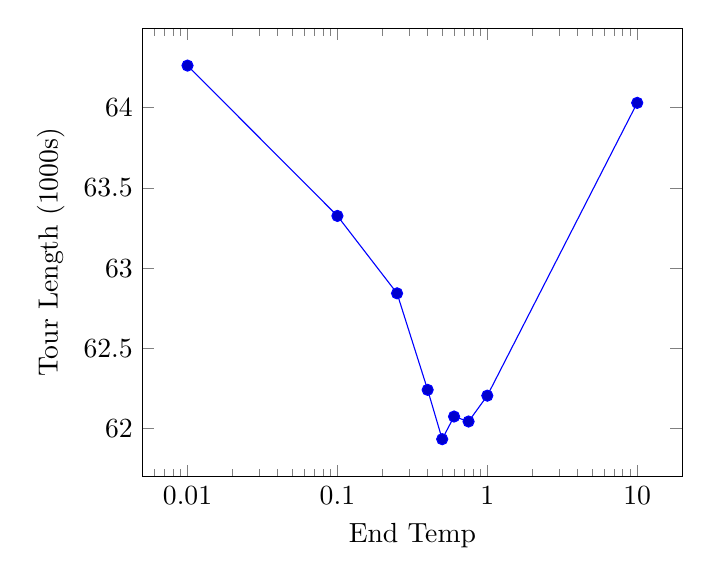
\begin{tikzpicture}
		\begin{axis}[
		%title = Effects of changing end temp,
		xlabel = {End Temp},
		ylabel = {Tour Length (1000s)},
		xmode=log,
		log ticks with fixed point,
		]
		\addplot coordinates {
			(0.01,64.261)
			(0.1,63.325)
			(0.25,62.843)
			(0.4,62.242)
			(0.5,61.935)
			(0.6,62.076)
			(0.75,62.045)
			(1,62.206)
			(10,64.029)
		};
		\end{axis}
		\end{tikzpicture}
	\end{tabu}
	
	%\vspace{-12pt}
	\subsection{Multithreading}	
	My implementation of Simulated Annealing supports multithreading. This was implemented by running the simulation on multiple threads and taking the best result. While running a simulation with $n$ steps on $m$ threads did improve the results, the results paled in comparison to a single-threaded run with $n \times m$ steps.
	
	To try and improve the quality of the results, the implementation was adjusted so that the current state was synchronised between the threads every $x$ steps. However, I could not find a happy medium between making $x$ too high and ruining the results, and having $x$ too low and wasting time managing threads constantly.
	
	On a larger graph, we could set $x$ quite high, and it would not adversely affect the results to the same extent.
	
	Alternative methods for multithreading could simply allow the threads to all work on the shared memory, updating the current state as they see fit. This could lead to race conditions, but that may not negatively impact results significantly. The worst case scenario would be that one thread would overwrite a better state with a worse state, which the simulated annealing algorithm does itself already.
	
	\subsection{Cooling Rate}
	The cooling rate can be changed via a parameter. After each step, the temperature is multiplied by the cooling factor ($1-rate$). A high cooling rate means that the simulation runs quicker but more coarsely, producing worse results. Conversely, low cooling rate means that the simulation takes more time, but produces better results. Runtime scales linearly with the number of steps.
	
	My implementation did not ask for Cooling Rate as a parameter, it instead asked for a number of steps and calculated the cooling rate as
	
	\begin{equation}
	\left({\frac{endTemp}{startTemp}}\right)^{\frac{1}{steps}}
	\end{equation}
	
	\begin{tabu}{X[c] X[c]}
		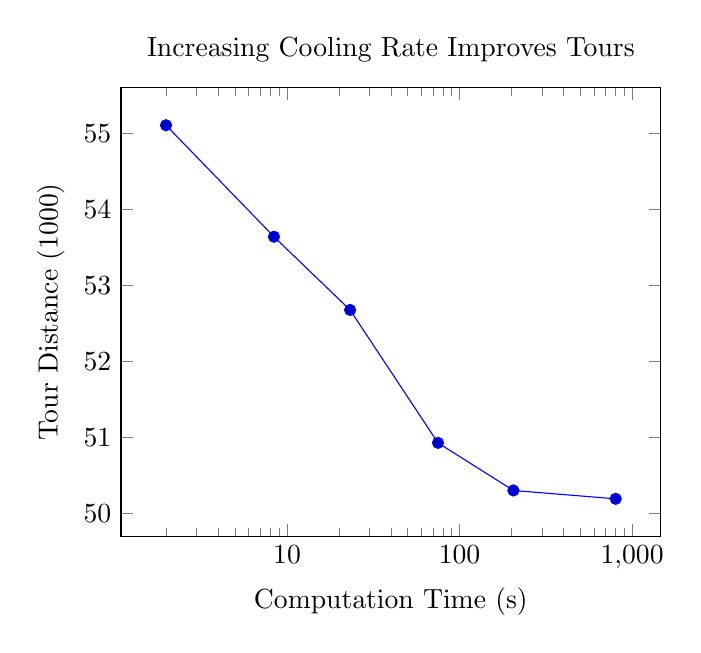
\begin{tikzpicture}
		\begin{axis}[
		title = Increasing Cooling Rate Improves Tours,
		xlabel = {Computation Time (s)},
		ylabel = {Tour Distance (1000)},
		xmode=log,
		log ticks with fixed point,
		]
		\addplot coordinates {
			(1.99,55.111)
			(8.40,53.643)
			(23.2,52.678)
			(75,50.928)
			(205,50.301)
			(803,50.191)
		};
		\end{axis}
		\end{tikzpicture}&
		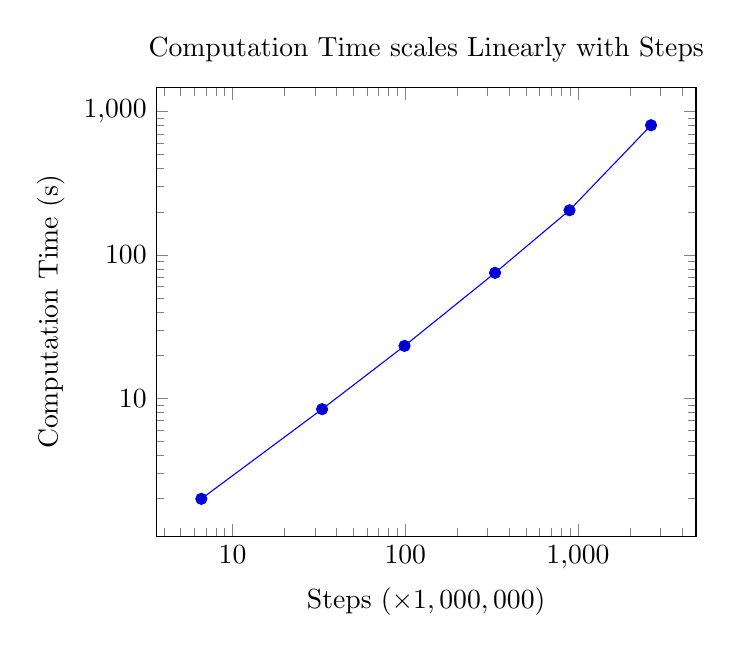
\begin{tikzpicture}
		\begin{axis}[
		title = Computation Time scales Linearly with Steps,
		xlabel = {Steps ($\times 1,000,000$)},
		ylabel = {Computation Time (s)},
		xmode=log,
		ymode=log,
		log ticks with fixed point,
		]
		\addplot coordinates {
			(6.6,1.99)
			(33,8.40)
			(99,23.2)
			(331,75)
			(893,205)
			(2648,803)
		};
		\end{axis}
		\end{tikzpicture}
	\end{tabu}
	
	%\vspace{-6pt}
	
	\section{Algorithm B: Ant Colony Optimisation}
	
	\subsection{Description}
	\begin{tabu}{p{10cm} X[c]}
		Ant Colony Optimisation simulates a number of ants moving around the graph. At each junction the ant chooses an edge to travel down using a weighted random selection. The weights for each edge are 
		
		\begin{equation}
		Pheromones^{2}*Length^{-2}
		\end{equation}
		
		Shorter edges are more desirable, as are edges with more pheromones. After each iteration, all ants deposit pheromones on the paths they travelled down. Pheromones then evaporate, with the pheromones on each edge being multiplied by a constant factor, specified by a parameter.
		&
		\rowcolors{0}{gray!25}{white}
		\begin{tabu}{|c c|}\hline
			\textbf{Nodes} & \textbf{Tour Length} \\
			12 & 56.0 \\
			17 & 1,444 \\
			21 & 2,549 \\
			26 & 1,575 \\
			42 & 1,322 \\
			48 & 12,702 \\
			58 & 25,855 \\
			175 & 21,770 \\
			180 & 1,950 \\
			535 & 50,124 \\\hline
		\end{tabu}
	\end{tabu}
	
	\subsection{Elite Ant}
	In each iteration, the best all-time ant was added to the ants to be processed. This means that the best all-time path has pheremones deposited onto it after each iteration, even if none of the generated ants chose that path. This should make the algorithm converge earlier.
	
	The algorithm with the Elite Ant consistently outperforms the algorithm without the Elite Ant. The Elite Ant algorithm ranges from slightly faster to much faster, with tour lengths almost identical.
	
	\begin{tabu}{X[c] X[c]}
		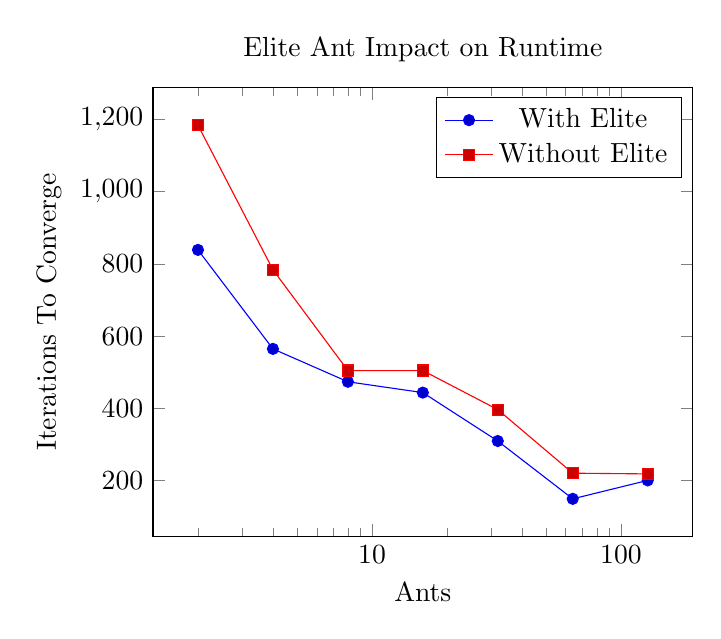
\begin{tikzpicture}
		\begin{axis}[
		title = Elite Ant Impact on Runtime,
		xlabel = {Ants},
		ylabel = {Iterations To Converge},
		xmode=log,
		log ticks with fixed point,
		]
		\addplot coordinates { %Elite
			(2,839)
			(4,565)
			(8,474)
			(16,444)
			(32,310)
			(64,150)
			(128,201)
		};
		\addlegendentry{With Elite}
		
		\addplot coordinates { %Without
			(2,1184)
			(4,784)
			(8,505)
			(16,505)
			(32,397)
			(64,221)
			(128,219)
		};
		\addlegendentry{Without Elite}
		\end{axis}
		\end{tikzpicture}&
		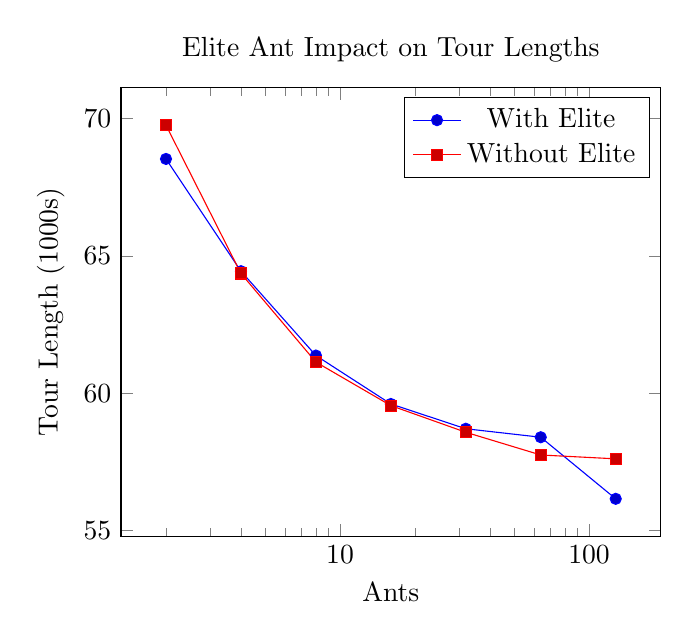
\begin{tikzpicture}
		\begin{axis}[
		title = Elite Ant Impact on Tour Lengths,
		xlabel = {Ants},
		ylabel = {Tour Length (1000s)},
		xmode=log,
		log ticks with fixed point,
		]
		\addplot coordinates { %Elite
			(2,68.531)
			(4,64.445)
			(8,61.375)
			(16,59.612)
			(32,58.710)
			(64,58.401)
			(128,56.159)
		};
		\addlegendentry{With Elite}
		
		\addplot coordinates { %Without
			(2,69.758)
			(4,64.362)
			(8,61.137)
			(16,59.553)
			(32,58.582)
			(64,57.755)
			(128,57.615)
		};
		\addlegendentry{Without Elite}
		\end{axis}
		\end{tikzpicture}
	\end{tabu}

	%\vspace{-12pt}
	\subsection{Multithreading}
	
	%\vspace{-12pt}
	\begin{tabu}{X[c] X[c]}	
		\begin{minipage}{\linewidth}
			Implementing multithreading into the ant colony optimisation was very easy and does not reduce the quality of the results whatsoever. When generating the ant population, we create multiple threads and ask each thread to create a portion of the ants. We then combine the generated lists and process the ants in a single-threaded manner.\\
			
			This works due to the fact that during ant generation, the shared resources are used in an entirely read-only fashion. The processing step could be run in parallel in future, but this will be difficult to implement due to shared resources being mutated.
		\end{minipage}
		
		&
		\begin{minipage}{\linewidth}
			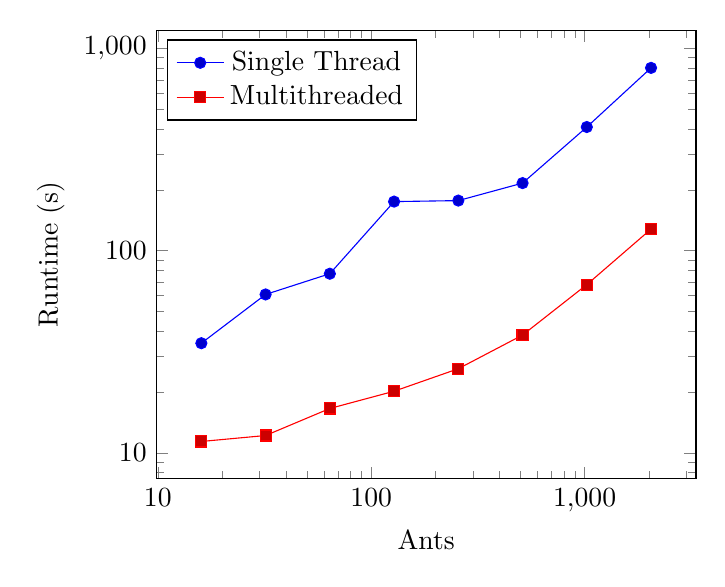
\begin{tikzpicture}
			\begin{axis}[
			xlabel = {Ants},
			ylabel = {Runtime (s)},
			xmode=log,
			ymode=log,
			log ticks with fixed point,
			legend style={at={(0.02,0.98)},anchor=north west},
			]
			\addplot coordinates { %ST
				(16,34.9)
				(32,60.8)
				(64,77)
				(128,175)
				(256,177)
				(512,216)
				(1024,409)
				(2048,802)
			};
			\addlegendentry{Single Thread}
			
			\addplot coordinates { %MT
				(16,11.4)
				(32,12.2)
				(64,16.6)
				(128,20.2)
				(256,26.1)
				(512,38.3)
				(1024,68)
				(2048,128)
			};
			\addlegendentry{Multithreaded}
			\end{axis}
			\end{tikzpicture}
		\end{minipage}
		\\
	\end{tabu}
	
	
	\subsection{Culling}
	\begin{tabu}{X[c] X[c]}
		\begin{minipage}{\linewidth}
			I attempted to improve performance of the ant colony optimisation by culling edges with sufficiently low desirability. This would mean that culled edges did not need to be considered when performing the weighted random selection.\\
			
			However, there was not a happy medium between having the culling happen too early (and therefore reduce the quality of the results) and having it happen too late (by which point the algorithm had already converged and we could have just ended it immediately).
		\end{minipage}&
		
		\begin{minipage}{\linewidth}
			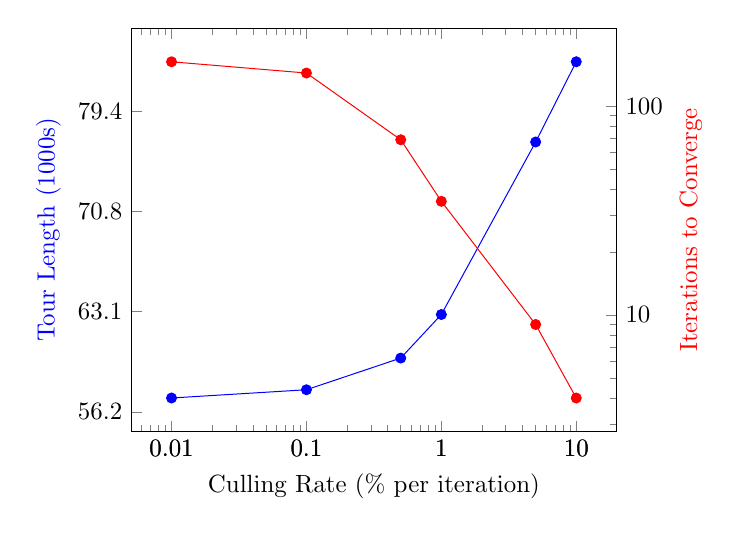
\begin{tikzpicture}[scale=0.9]
			\begin{axis}[
			xlabel = {Culling Rate (\% per iteration)},
			ylabel = {\color{blue}Tour Length (1000s)},
			axis y line*=left,
			ylabel near ticks,
			xmode=log,
			ymode=log,
			log ticks with fixed point,
			]
			\addplot[blue,mark=*] coordinates {
				(0.01,57.154)
				(0.1,57.700)
				(0.5,59.838)
				(1,62.910)
				(5,76.699)
				(10,84.099)
			};
			\end{axis}
			
			\begin{axis}[
			ylabel = {\color{red}Iterations to Converge},
			axis y line*=right,
			ylabel near ticks,
			xmode=log,
			ymode=log,
			log ticks with fixed point,
			]
			\addplot[red,mark=*] coordinates { %ST
				(0.01,163)
				(0.1,144)
				(0.5,69)
				(1,35)
				(5,9)
				(10,4)
			};
			\end{axis}
			\end{tikzpicture}
		\end{minipage}
	\end{tabu}
	
	\section{General}
	
	\subsection{Fast Triangular Array}
	Originally, the matrix was stored using a HashMap of unordered pairs. This was incredibly slow. Accessing an edge's length meant creating a new object, hashing it, then retrieving that from the hashtable. I changed my approach, creating an array of $size=nodes^2$. When requesting position $(x,y)$, it retrieved position $x_2 \times nodes + y_2$ where $x_2$ was $min(x,y)$ and $y_2$ was $max(x,y)$. This reflects the graph's directionless nature.
	
	\subsection{Grouping}
	\begin{tabu}{X[c] X[c]}
		\begin{minipage}{\linewidth}
			By grouping nodes that are near each other, we can break the TSP into multiple smaller TSPs. This can be done repeatedly, using the groups of this layer as the nodes of the layer above, until the uppermost level only contains one node. We then solve the top layer, which is trivial, followed by repeatedly solving the group represented by each node in the tour, replacing it with the solution of the layer below. When all nodes in the tour are part of the bottom layer, we are finished.\\
			
			The main challenges with this technique are how to group the nodes, and how to calculate the distances between nodes in the new network. Both of these problems are made much easier if the initial network exists in euclidean space. The method used involves iteratively building a group from a start node, where in each iteration we add the node with the lowest equivalent electrical resistance to the start node. The distances between nodes were calculated as the average distance between nodes in the two groups.\\
			
			This algorithm tends to give approximate results very quickly, and significantly outperforms other algorithms when given less than a second to run. On the 535 node network, it was found that the grouping algorithm with Simulated Annealing could produce a tour of 61.8k in 0.15 seconds, whereas it took 0.5 seconds for standard Simulated Annealing to beat this score. On a network of 3000 nodes, this crossover point was increased to 1.5 seconds, and it should increase more as the size of the network increases.\\
			
			This approach is not yet optimised, and could see significant improvements. Specifically, it is not known what impact allocating more time to the initial grouping could achieve. The current grouping implementation is not capable of this. Allowing extra time for intra-group solving does not tend to improve the results much.\\
		\end{minipage}&
		
		\begin{minipage}{\linewidth}
			\begin{center}
				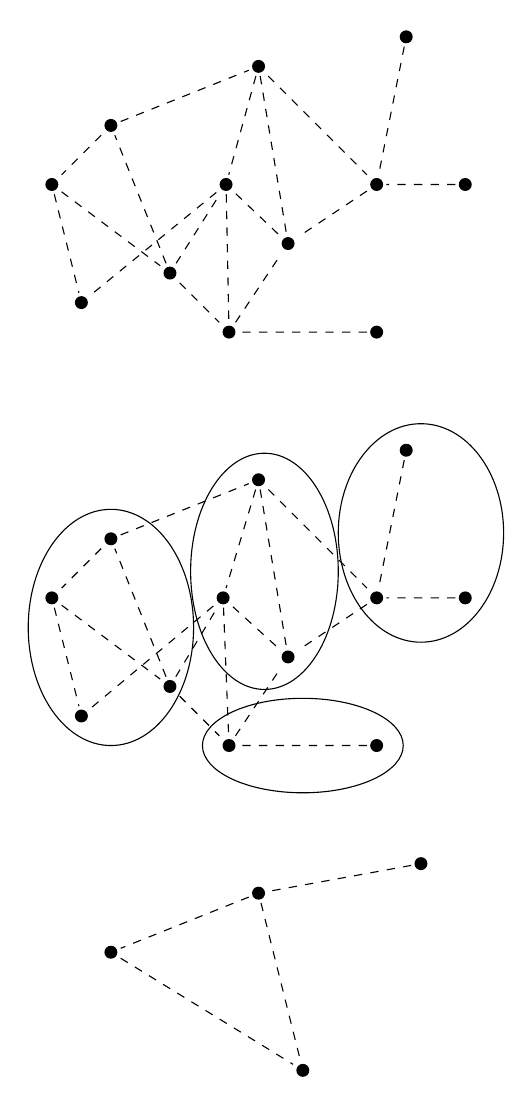
\begin{tikzpicture}[rotate=180,scale=0.75]
				\node (v4) at (-4,-20.5) {};
				\node (v5) at (-4.95,-22) {};
				\node (v7) at (-2,-22) {};
				\node (v8) at (-2.5,-20) {};
				\node (v6) at (-3,-23) {};
				\node (v2) at (-5,-19.5) {};
				\node (v11) at (-7.5,-22) {};
				\node (v9) at (-5.5,-24) {};
				\node (v3) at (-6,-21) {};
				\node (v1) at (-7.5,-19.5) {};
				\node (v10) at (-8,-24.5) {};
				\node (v12) at (-9,-22) {};
				
				\draw (v4) [fill=black] ellipse (0.1 and 0.1);
				\draw (v5) [fill=black] ellipse (0.1 and 0.1);
				\draw (v7) [fill=black] ellipse (0.1 and 0.1);
				\draw (v8) [fill=black] ellipse (0.1 and 0.1);
				\draw (v6) [fill=black] ellipse (0.1 and 0.1);
				\draw (v2) [fill=black] ellipse (0.1 and 0.1);
				\draw (v11) [fill=black] ellipse (0.1 and 0.1);
				\draw (v9) [fill=black] ellipse (0.1 and 0.1);
				\draw (v3) [fill=black] ellipse (0.1 and 0.1);
				\draw (v1) [fill=black] ellipse (0.1 and 0.1);
				\draw (v10) [fill=black] ellipse (0.1 and 0.1);
				\draw (v12) [fill=black] ellipse (0.1 and 0.1);
				
				\draw [dashed] (v1) edge (v2);
				\draw [dashed] (v2) edge (v3);
				\draw [dashed] (v4) edge (v5);
				\draw [dashed] (v4) edge (v6);
				\draw [dashed] (v7) edge (v8);
				\draw [dashed] (v7) edge (v4);
				\draw [dashed] (v5) edge (v2);
				\draw [dashed] (v4) edge (v2);
				\draw [dashed] (v9) edge (v5);
				\draw [dashed] (v10) edge (v11);
				\draw [dashed] (v12) edge (v11);
				\draw [dashed] (v11) edge (v3);
				\draw [dashed] (v9) edge (v11);
				\draw [dashed] (v6) edge (v7);
				\draw [dashed] (v5) edge (v8);
				\draw [dashed] (v5) edge (v3);
				\draw [dashed] (v9) edge (v3);
				\draw [dashed] (v6) edge (v9);
				
				\node (v4) at (-4,-13.5) {};
				\node (v5) at (-4.9,-15) {};
				\node (v7) at (-2,-15) {};
				\node (v8) at (-2.5,-13) {};
				\node (v6) at (-3,-16) {};
				\node (v2) at (-5,-12.5) {};
				\node (v11) at (-7.5,-15) {};
				\node (v9) at (-5.5,-17) {};
				\node (v3) at (-6,-14) {};
				\node (v1) at (-7.5,-12.5) {};
				\node (v10) at (-8,-17.5) {};
				\node (v12) at (-9,-15) {};
				
				\draw (v4) [fill=black] ellipse (0.1 and 0.1);
				\draw (v5) [fill=black] ellipse (0.1 and 0.1);
				\draw (v7) [fill=black] ellipse (0.1 and 0.1);
				\draw (v8) [fill=black] ellipse (0.1 and 0.1);
				\draw (v6) [fill=black] ellipse (0.1 and 0.1);
				\draw (v2) [fill=black] ellipse (0.1 and 0.1);
				\draw (v11) [fill=black] ellipse (0.1 and 0.1);
				\draw (v9) [fill=black] ellipse (0.1 and 0.1);
				\draw (v3) [fill=black] ellipse (0.1 and 0.1);
				\draw (v1) [fill=black] ellipse (0.1 and 0.1);
				\draw (v10) [fill=black] ellipse (0.1 and 0.1);
				\draw (v12) [fill=black] ellipse (0.1 and 0.1);
				
				\draw [dashed] (v1) edge (v2);
				\draw [dashed] (v2) edge (v3);
				\draw [dashed] (v4) edge (v5);
				\draw [dashed] (v4) edge (v6);
				\draw [dashed] (v7) edge (v8);
				\draw [dashed] (v7) edge (v4);
				\draw [dashed] (v5) edge (v2);
				\draw [dashed] (v4) edge (v2);
				\draw [dashed] (v9) edge (v5);
				\draw [dashed] (v10) edge (v11);
				\draw [dashed] (v12) edge (v11);
				\draw [dashed] (v11) edge (v3);
				\draw [dashed] (v9) edge (v11);
				\draw [dashed] (v6) edge (v7);
				\draw [dashed] (v5) edge (v8);
				\draw [dashed] (v5) edge (v3);
				\draw [dashed] (v9) edge (v3);
				\draw [dashed] (v6) edge (v9);
				\draw (-8.25,-16.1) node (v21) {} ellipse (1.4 and 1.85);
				\draw (-6.25,-12.5) node (v22) {} ellipse (1.7 and 0.8);
				\draw (-3,-14.5) node (v24) {} ellipse (1.4 and 2);
				\draw (-5.6,-15.45) node (v23) {} ellipse (1.25 and 2);
				
				\node (v13) at (-8.25,-10.5) {};
				\node (v14) at (-5.5,-10) {};
				\node (v16) at (-3,-9) {};
				\node (v15) at (-6.25,-7) {};
				
				\draw (v13) [fill=black] ellipse (0.1 and 0.1);
				\draw (v14) [fill=black] ellipse (0.1 and 0.1);
				\draw (v16) [fill=black] ellipse (0.1 and 0.1);
				\draw (v15) [fill=black] ellipse (0.1 and 0.1);
				
				\draw [dashed] (v13) edge (v14);
				\draw [dashed] (v14) edge (v15);
				\draw [dashed] (v16) edge (v15);
				\draw [dashed] (v14) edge (v16);
				\end{tikzpicture}
				
				\vspace{12pt}
				
				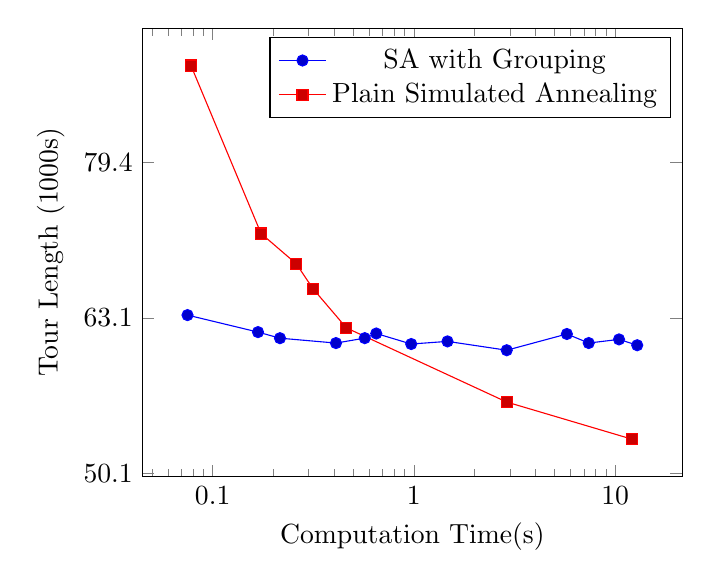
\begin{tikzpicture}
				\begin{axis}[
				xlabel = {Computation Time(s)},
				ylabel = {Tour Length (1000s)},
				xmode=log,
				ymode=log,
				log ticks with fixed point,
				]
				\addplot coordinates { %Grouping
					(0.075,63.388)
					(0.168,61.811)
					(0.216,61.256)
					(0.41,60.815)
					(0.57,61.262)
					(0.65,61.684)
					(0.97,60.731)
					(1.469,60.966)
					(2.894,60.176)
					(5.759,61.638)
					(7.394,60.822)
					(10.46,61.147)
					(12.88,60.624)
				};
				\addlegendentry{SA with Grouping}
				
				\addplot coordinates { %Without
					(0.078,91.704)
					(0.174,71.522)
					(0.26,68.402)
					(0.316,65.884)
					(0.462,62.2)
					(2.89,55.733)
					(12.11,52.753)
				};
				\addlegendentry{Plain Simulated Annealing}
				\end{axis}
				\end{tikzpicture}
			\end{center}
		\end{minipage}
		\\
	\end{tabu}
	
\end{document}